\documentclass{beamer}

\usepackage{mjclectureslides}

\definecolor{Dblue}{rgb}{.255,.41,.884}

\title[$\R$]{Introduction to Analysis: \\ The Real Numbers}
%\author[Prof. Michael Carlisle]{Prof. Michael Carlisle} 
%\institute{Baruch College, CUNY}
%\date{Fall 2017}
\date{}

\begin{document}

\frame{\titlepage}


\frame{ \frametitle{Well ordering principle}

\begin{center}
\textbf{Every \emph{nonempty} set of natural numbers $S$,
\[ \emptyset \neq S \subseteq \mathbb{N}, \] 
has a smallest element.}
\end{center}

\vspace{5mm}

\begin{notenote}
The empty set $\emptyset$, having no elements, has no \emph{smallest} element.
\end{notenote}

\vspace{5mm}

Otherwise, this seems like an obvious statement, because you've been trained on the \emph{well-ordering} property of the natural numbers $\mathbb{N}$ since you were very young. 

}



\frame{ \frametitle{Well ordering principle: countable sets}


\begin{prop}
Any subset $C \subseteq \N$ is countable (finite or infinite).
\end{prop}

\vspace{5mm}

\pf By the Well Ordering Principle, select the smallest element of $C$, call it entry 1 ($c_1$) in the list. 

\vspace{5mm}

The next smallest is entry 2 ($c_2$). Continue. $\blacksquare$

}


\frame{ \frametitle{Well ordering principle: Fractions have lowest terms}


\begin{thm}
Every positive rational number $q \in \mathbb{Q}^+ = \{ q \in \mathbb{Q}: \, q > 0 \}$ has a representation in \textbf{lowest terms}, i.e. a form 

\[ q = \frac{m}{n}, \,\, m, n \in \mathbb{N} \] 

\vspace{3mm}

where $m$ and $n$ have no common factors. 
\end{thm}

\vspace{3mm}

\pf We will prove by contradiction. 

\vspace{3mm}

Let $C$ be the set of positive integers that are numerators $m$ of fractions $\frac{m}{n}$ that do \emph{not} have a form in lowest terms. 

}


\frame{ \frametitle{Well ordering principle: Fractions have lowest terms}

\[ C = \left\{m \in \N: \,\, \frac{m}{n} \in \Q, \,\, \frac{m}{n} \text{ has \emph{no} lowest terms}\right\} \]

\vspace{3mm}

Assume $C$ is nonempty. %\textcolor{red}{[$\sim Q$]} 

\vspace{5mm}

Then, by Well Ordering, there is a smallest element $m_0 \in C$. 

\vspace{5mm}

(This is considered a counterexample to the proposition. \\
We will show that there are none.)
%\textcolor{red}{[$P \implies \sim Q$]} 

}


\frame{ \frametitle{Well ordering principle: fractions have lowest terms}

Let $n_0 \in \mathbb{N}$ be a denominator such that $\frac{m_0}{n_0}$ has no lowest terms. 

\vspace{5mm}

Thus, $\frac{m_0}{n_0}$ is not in lowest terms, so a common factor can be divided out. Call a possible common factor $p \geq 2$. Thus, 
\[ \frac{ \frac{m_0}{p} }{ \frac{n_0}{p} } = \frac{m_0}{n_0}. \]
Thus, $\frac{\frac{m_0}{p} }{ \frac{n_0}{p}}$ also has no lowest terms form, and so $\frac{m_0}{p} \in C$. 

\vspace{5mm}

But $\frac{m_0}{p} < m_0$, and we assumed $m_0$ was the smallest nonnegative integer in $C$. This is a contradiction $\contra$.  Therefore, $C = \emptyset$. $\blacksquare$

}


\frame{ \frametitle{Well ordering principle-based proofs, Induction}

Proofs using the well ordering principle often go for a contradiction, showing that there are no elements that satisfy a certain property. 

\vspace{5mm}

On the other hand, the \textbf{Principle of Mathematical Induction} (or, simply, \textbf{induction}) is a family of techniques for direct, often constructive, discrete mathematics\footnote{which is why the technique lends itself so well to computer science}. 

}


\frame{ \frametitle{Well ordering principle-based proofs, Induction}

The idea: $p(n)$ is a predicate for $n \in I$, some discrete index set: 

\[ I = \{k, k+1, k+2, ...\} \text{ for some } k \in \mathbb{Z}. \text{  (Usually, } k = 0 \text{ or } 1.) \]

\vspace{5mm}

You wish to prove 

\[  \forall n \geq k, \, p(n). \]

}


\frame{ \frametitle{Induction}

How we do this: 

\vspace{3mm}

\begin{enumerate}
\item Start with a \emph{base case}, $p(k)$, which should be easy to prove. (It might even seem \emph{too} easy.)
\vspace{3mm}
\item Take the \emph{inductive step}: Assume $p(n)$ for a fixed $n \geq k$. \\
(This is called the \emph{inductive hypothesis}.)

\vspace{3mm}

Use $p(n)$ to prove $p(n+1)$. 
\end{enumerate}

}


\frame{ \frametitle{Induction}

The result is the Method of Induction starting at $k \in \Z$ for $p(n)$:  

\vspace{3mm}

\[ p(k) \land (\forall n \geq k, \,  p(n) \implies p(n+1)) \implies  \forall n \geq k, \, p(n). \]

\vspace{5mm}

We can prove that induction works using Well Ordering. 

\vspace{5mm}

We'll assume for simplicity that $k=1$.

}


\frame{ \frametitle{Induction is Provable via Well Ordering}

\begin{thm} \textbf{(Induction)} Let $p(n)$ be a predicate for $n \in \N$. Then 
\[ p(1) \land (\forall n \geq 1, \,  p(n) \implies p(n+1)) \implies  \forall n \geq 1, \, p(n). \]
\end{thm}

\pf Let 
\[ S = \{ n \in \N: \, p(n) \text{ is false}\}. \]

We assume that $S \neq \emptyset$, and the following implication is true:
\[ p(1) \land (\forall n \geq 1, \,  p(n) \implies p(n+1)). \] 

\vspace{5mm}

We will prove, for a contradiction, that $S = \emptyset$. 

}


\frame{ \frametitle{Induction is Provable via Well Ordering}

$S \subseteq \N$, so by Well Ordering, $S$ has a smallest element. Call it $m$. 

\vspace{5mm}

$m \geq 2$ since we assume $p(1)$ is true, so $1 \not \in S$. 

\vspace{5mm}

If $p(m)$ is false, and the implication $p(m-1) \implies p(m)$ is true, then by the truth table for $p(m-1) \implies p(m)$, we know that $p(m-1)$ must also be false\footnote{Check this directly by writing out the truth table.}.

\vspace{5mm}

Hence, $m-1 \in S$, contradicting $m$ as the smallest element of $S$. $\contra$ \,\, $\therefore$ $S$ is empty.  $\blacksquare$

}


\frame{ \frametitle{Induction: Gauss' trick}

The canonical first example in induction is \textbf{Gauss' trick}. 
\begin{thm}
\[ \forall n \in \mathbb{N}, \sum_{i=1}^n i = \frac{n(n+1)}{2}. \]
\end{thm}

\pf We prove by induction. First, we show the base case $n=1$: 
\[ \sum_{i=1}^1 i = 1 = \frac{1(2)}{2}. \,\, \checkmark\]

Now, assume the inductive hypothesis $\color{red}{\sum_{i=1}^n i = \frac{n(n+1)}{2}}$\color{black}. Then, 
\[\sum_{i=1}^{n+1} i = \color{red}{\sum_{i=1}^{n} i}\color{black} + (n+1) = \color{red}{\frac{n(n+1)}{2}}\color{black} + \frac{2(n+1)}{2} = \frac{(n+1)(n+2)}{2}. \,\,\,\,\, \blacksquare \]

}


\frame{ \frametitle{Strong induction}

\textbf{Strong induction} is another form of induction (logically equivalent to ``regular'' induction) which allows you to assume \emph{all} predicates before the given ``new'' one in your inductive step. That is, 

\vspace{5mm}

\begin{enumerate}
\item Start with a \emph{base case}, $p(k)$, which should be easy to prove. (It might even seem \emph{too} easy.)
\vspace{3mm}
\item Take the \emph{strong inductive step}: Assume 
\[ p(k), p(k+1), ..., p(n-1), p(n) \] 
for a fixed $n \in I$. \\
(This is called the \emph{strong inductive hypothesis}.) 

\vspace{3mm}

Use as many of these as you like to prove $p(n+1)$. 
\end{enumerate}

}


\frame{ \frametitle{Strong induction}

This is represented logically by 
\begin{align*} 
\bigg( p(k) \, \land & \bigg[ (p(k) \land p(k+1) \land \cdots \land p(n)) \implies p(n+1) \bigg] \bigg) \\
 & \implies \forall n \geq k,  \, p(n).
\end{align*}

}



\frame{ \frametitle{Strong induction: $n \in \N$, $n > 1$ has a prime factorization }

\begin{prop}
$\forall n \in \mathbb{N}$, $n > 1$ $\implies n$ is a product of primes.
\end{prop}

%\onslide<2->
\vspace{3mm}

\pf We will use strong induction. \\
First, the base case: $n=2$ is clearly a (product of) prime(s).

\color{red}Next, the inductive step: assume that $2, 3, ..., n-1, n$ are all products of primes. 
\color{black}
%\onslide<3->
\vspace{3mm}

There are two possible cases for $n+1$: 
\begin{itemize}
\item $n+1$ is prime itself: nothing to show.
\item $n+1$ is composite: then $\exists m, q \in \mathbb{N}:  2 \leq m \leq q < n+1$ such that $n+1 = mq$. 
\color{red}Since $m, q \leq n$, then each is known to be a product of primes. \color{black}Therefore, $n+1$ is a product of primes since it is a product of $m$ and $q$. $\blacksquare$
\end{itemize}

}


\frame{ \frametitle{Well ordering principle vs induction}

Using the well ordering principle is also equivalent to using induction, but they have a difference in style.

\vspace{5mm}

Well ordering principle-based proofs deal with finding a \emph{counterexample} $n \in I$ to a predicate $p(n)$ being true. 

\vspace{5mm}

In particular, attempt to find the minimum possible $n$ such that $p(n)$ is false. 

\vspace{5mm}

Finding that one does not exist results in the conclusion that $p(n)$ is always true.

}


\frame{ \frametitle{Well ordering principle vs induction}

Induction proofs first show that a base case is true, then show that each successive predicate is also true because of it.

\vspace{5mm}

\textbf{Guideline}: If you want to show a contradiction, use well ordering \\(i.e. ``there are no values that do \emph{not} satisfy this property''). 

\vspace{5mm}

If you wish to prove directly, use induction \\(i.e. ``each of these values satisfies this property'').

}


\frame{ \frametitle{Well ordering principle vs induction: Gauss' trick}

We will re-prove \textbf{Gauss' trick} using the well ordering principle.

\vspace{5mm}

\begin{prop} 
$\forall n \in \mathbb{N}, \sum_{i=1}^n i = \frac{n(n+1)}{2}$.
\end{prop}

\vspace{5mm}

\pf We prove by well ordering. \\Let $S$ be the set of $n \in \mathbb{N}$ such that Gauss' trick does not work. 

\vspace{3mm}

Assume (for a contradiction) that $S$ is nonempty and, \\by well ordering, let $m$ be the smallest element of $S$. 

\vspace{3mm}

Thus, 
\[ \sum_{i=1}^m i \neq \frac{m(m+1)}{2}. \] 

}


\frame{ \frametitle{Well ordering principle vs induction: Gauss' trick}

Clearly, $m > 1$ since $1 = \frac{1(2)}{2}$. But in that case, 

\begin{align*} 
\sum_{i=1}^{m-1} i & = \frac{(m-1)(m)}{2} \\
\sum_{i=1}^{m} i & = \sum_{i=1}^{m-1} i + m \\
 & = \frac{(m-1)(m)}{2} + m = \frac{m(m+1)}{2}.
\end{align*} 

\vspace{3mm}

Thus, $m \not \in S$. $\contra$ \,\,\, $\blacksquare$

}


\frame{ \frametitle{$\mathbb{R}$ = ``the set of lengths with a direction (sign)''} 

The set of real numbers $\mathbb{R}$ can be described as 

\vspace{2mm}

\begin{center}
``all the lengths possible (positive and negative) on the number line, relative to a fixed point called zero (0).''
\end{center}

\vspace{3mm}

This induces a \textbf{total ordering}\footnote{This is in comparison with a \emph{partial ordering}, under which all pairs of elements can not necessarily be compared.}
 on the set, in which every pair of two distinct elements can be compared: this ordering is called \\
\begin{center}
``less than'' ($<$).
\end{center}


}


\frame{ \frametitle{$\mathbb{R}$ = ``the only complete ordered field''} 

The set of \textbf{real numbers} is \textbf{the only complete ordered field}. 

\vspace{5mm}

\begin{itemize}
\item ``only" in the sense that any other complete ordered field can be set in 1-1 correspondence with $\R$; 

\vspace{3mm}

\item ``complete'' in the sense of containing limits of sequences \\(we will address this in the next section);

\vspace{3mm}

\item ``ordered'' in the sense of the total order $<$;

\vspace{3mm}

\item ``field'' will be defined now, in terms of the \textbf{field axioms}, which must hold for any set to be called a \textbf{field} \\(in abstract algebra terms).
\end{itemize}


}


\frame{ \frametitle{Field Axioms of Real Numbers}

The real numbers $\R$ have two binary operations, $+$ (``addition'') and $\cdot$ (``multiplication'') which have the following properties: 

\vspace{5mm}

\begin{itemize}
\item[(A,M1)] $+$ and $\cdot$ are \textbf{closed} in $\R$, and consistent: 
\begin{align*}
x, y \in \R & \implies x+y, xy \in \R \\
x=w, \, y=z & \implies x+y = w+z, \, xy = wz
\end{align*}

\item[(A,M2)] $+$, $\cdot$ are \textbf{commutative} in $\mathbb{R}$: 
\[ x+y = y+x, \,\, xy = yx \]
\end{itemize}


}


\frame{ \frametitle{Field Axioms of Real Numbers}

\begin{itemize}
\item[(A,M3)] $+$, $\cdot$ are \textbf{associative} in $\mathbb{R}$: 
\[ (x+y)+z = x+(y+z), \,\, (xy)z = x(yz) \]

\vspace{3mm}

\item[(DL)] \textbf{distributive law}: $x(y+z) = xy + xz$
\end{itemize}

}


\frame{ \frametitle{Field Axioms of Real Numbers}

\begin{itemize}
\item[(A4)] $\exists !$ number\footnote{$\exists !$ denotes \emph{unique existence}; only one of this type of object exists in $\R$!} $0 \in \R$, the \textbf{additive identity}, such that
\[ \forall x \in \mathbb{R}, \,\, x + 0 = 0 + x = x \]

\vspace{3mm}

\item[(M4)] $\exists !$ number $1 \in \R$, the \textbf{multiplicative identity}, such that
\[ 1 \neq 0 \text{ and } x \cdot 1 = 1 \cdot x = x \]
\end{itemize}


}


\frame{ \frametitle{Field Axioms of Real Numbers}

\begin{itemize}
\item[(A5)] For each $x \in \mathbb{R}$, $\exists a \in \mathbb{R}$, the \textbf{additive inverse} of $x$, denoted $a = -x$, such that 
\[ x + a = a + x = 0 \]

\vspace{3mm}

\item[(M5)] For each $x \in \mathbb{R} \setminus \{0\}$, $\exists b \in \mathbb{R}$, the \textbf{multiplicative inverse} of $x$, denoted $b = \frac{1}{x} = x^{-1}$, such that 
\[ xb = bx = 1 \]
\end{itemize}

}


\frame{ \frametitle{Inverse Operations of Real Numbers}

We then define the inverse operations of addition and multiplication (called \textbf{subtraction} and \textbf{division}, of course) by \emph{non-commutative} combination with inverse second elements. 

\vspace{5mm}

The operation of ``subtraction'' of $x \in \R$ by $y \in \R$ is defined by 
\[ x - y = x + (-y). \]

The operation of ``division'' of $x \in \R$ by $y \in \R \setminus \{0\}$ is defined by 
\[ x \div y = x \cdot y^{-1}. \]

}


\frame{ \frametitle{Order Axioms of the Real Numbers}

In addition to the field axioms, the real numbers have \textbf{order axioms} that apply to the relation we have called $<$. 

\vspace{5mm}

\begin{itemize}
\item[(O1)] \textbf{Trichotomy} \, \\
$\forall x, y \in \mathbb{R}$, exactly one of these three statements is true: 
\[ x < y, \,\, x = y, \,\, y < x. \]
We will also define the notation $x > y$ for the case $y < x$, \\ i.e. $>$ is the inverse relation of $<$.
\end{itemize}

%\vspace{3mm}

%Note that trichotomy is the same as saying $<$ is antisymmetric and irreflexive. Add in transitivity (we will) and $<$ is a \emph{strong total order}.

}


\frame{ \frametitle{Order Axioms of the Real Numbers}

\begin{itemize}
\item[(O2)] \textbf{Transitivity } 
\[ \forall x, y, z \in \R, \,\, x < y \text{ and } y < z \implies x < z. \]

\vspace{3mm}

\item[(O3)] \textbf{Shift Invariance } 
\[ \forall x, y, z \in \R, \,\, x < y \implies x+z < y+z. \]

\vspace{3mm}

\item[(O4)] \textbf{Positive Scale Invariance } 
\[ \forall x, y, z \in \R, \,\, x < y \text{ and } 0 < z \implies xz < yz. \]
\end{itemize}

}


\frame{ \frametitle{Order Axioms of the Real Numbers}

A real number $x \in \mathbb{R}$ is called 

\vspace{3mm}

\begin{itemize}
\item \textbf{positive} if $x > 0$, \textbf{nonnegative} if $x \geq 0$

\vspace{3mm}

\item \textbf{negative} if $x < 0$, \textbf{nonpositive} if $x \leq 0$
\end{itemize}

\vspace{3mm}

where the relations $\leq$ and $\geq$ are defined in the obvious way: 

\vspace{3mm}

\begin{itemize}
\item $x \leq y$ $\iff$ $(x < y)$ or $(x = y)$

\vspace{3mm}

\item $x \geq y$ $\iff$ $(y < x)$ or $(x = y)$
\end{itemize}

}


\frame{ \frametitle{$\R$ is not the only field.}

A number system $F$ with the following properties is called a \textbf{field}: 

\vspace{3mm}

\begin{itemize}
\item[(A,M1)] $F$ has two binary arithmetic operations \\
(which we'll call $+$ and $\cdot$) under which $F$ is \emph{closed}, \\meaning that, if $a, b \in F$, then $a+b, a \cdot b \in F$ as well.

\vspace{3mm}

\item[(A,M2)] $+$ and $\cdot$ are commutative.

\vspace{3mm}

\item[(A,M3)] $+$ and $\cdot$ are associative.

\vspace{3mm}

\item[(DL)] $+$ and $\cdot$ are distributive. 

\vspace{3mm}

\item[(A,M4)] $F$ has a unique \textbf{additive identity} (0) \\and \textbf{multiplicative identity} (1).

\vspace{3mm}

\item[(A,M5)] $F$ contains \textbf{additive inverses} \\and \textbf{multiplicative inverses} for all its nonzero elements.
\end{itemize}

}


\frame{ \frametitle{Inequalities: the ordering of $\mathbb{R}$}

Here are some properties of real number inequalities: 

\vspace{3mm}

\begin{prop}
$a < b \implies 0 < b-a$. 
\end{prop}

\vspace{3mm}

\pf By (O3), 
\[ a < b \implies a + (-a) < b + (-a) \implies 0 < b - a. \,\, \blacksquare \]

}


\frame{ \frametitle{Inequalities: the ordering of $\mathbb{R}$}

\begin{prop}
If $a < b$ and $c < d$, then $a + c < b + d$. 
\end{prop}

\vspace{3mm}

\pf By (O3), 
\[ a < b \implies a + c < b + c \text{ and } c < d \implies c + b < d + b. \]
But, by (A2), 
\[ b + c = c + b \text{ and } d + b = b + d. \]
Therefore, 
\[ a + c < b + c < b + d. \,\, \blacksquare \]

}


\frame{ \frametitle{Inequalities: the ordering of $\mathbb{R}$}


\begin{prop}
$x > y \iff -x < -y$. 
\end{prop}

\vspace{3mm}

\pf Suppose $x \neq y$. Further, suppose $x > y$ and $-x > -y$. Then, by the previous proposition, 
\[ x + (-x) > y + (-y) \implies 0 > 0, \]
which is a contradiction. Hence, one of the inequalities is false. $\blacksquare$

\vspace{3mm}

\begin{cor}
$x > 0$ $\implies -x < 0$.
\end{cor}

}


\frame{ \frametitle{More inequality properties}

\begin{prop}
$x \neq 0$ $\implies x^2 > 0$.
\end{prop}

\vspace{3mm}

\pf Two cases: 
\begin{align*}
I. \,\, x > 0 & \implies x^2 > x(0) = 0 \text{ by positive scale invariance (O4).} \\
II.\,\,  x < 0 & \implies -x > 0 \text{ by the previous proposition } \\
 & \implies (-x)(-x) = x^2 > 0(-x) = 0. \,\, \blacksquare
\end{align*}

}


\frame{ \frametitle{More inequality properties}

\begin{prop}
$0 < 1$. 
\end{prop}

\vspace{3mm}

\pf We are given $0 \neq 1$ in (M4). 

\vspace{3mm}

If $0 > 1$, then $-0 = 0 < -1$, which implies by the previous proposition that $0 < (-1)(-1) = 1$. 

\vspace{3mm}

$0 > 1 \implies 0 < 1$ is a contradiction of trichotomy. 

\vspace{3mm}

$\therefore 0 \not > 1$, and so $0 < 1$ is the only one of the three that holds. $\blacksquare$

}


\frame{ \frametitle{Even more inequality properties}

\begin{prop}
$u > v > 0$ $\implies u^2 > v^2$. 
\end{prop}

\vspace{3mm}

\pf By scale invariance, 
\[ u > v \implies u^2 > uv \text{ and } uv > v^2. \]
Combining these two via transitivity, we get $u^2 > v^2$.  $\blacksquare$

}


\frame{ \frametitle{Even more inequality properties}

\begin{prop}
$x > 0$ $\implies \frac{1}{x} > 0$.
\end{prop}

\vspace{5mm}

\pf $\frac{1}{x} \neq 0$, so for a contradiction, assume $x > 0$ and $\frac{1}{x} < 0$. 

\vspace{3mm}

Then $x \cdot \frac{1}{x} = 1 < 0$. $\contra$ 
  $\blacksquare$


}


\frame{ \frametitle{Even more inequality properties}

\begin{prop}
If $xy = 0$ and $y \neq 0$, then $x = 0$. 
\end{prop}

\vspace{5mm}

\pf $y \neq 0$ and $y \in \R$ $\implies$ $y^{-1} \in \R$, $y^{-1} \neq 0$. Then, 

\vspace{3mm}

\[ xy = 0 \implies xyy^{-1} = 0y^{-1} \implies x \cdot 1 = x = 0. \,\, \blacksquare \]

}


\frame{ \frametitle{A helpful analysis bounding theorem}

\begin{thm}
Let $x, y \in \R$ \, such that \, $\forall \ve > 0$, $x \leq y + \ve$. Then $x \leq y$. 
\end{thm}

\vspace{3mm}

\pf We will prove the contrapositive. Suppose $x > y$. 

\vspace{3mm}

(We need to show $\exists \ve > 0$ such that $x > y + \ve$.)

\vspace{3mm}

Let $\ve = \frac{x-y}{2}$. We know that 
\[ x > y \text{ and } \frac{1}{2} > 0 \implies x-y > 0 \implies \ve > 0. \] 
Thus, 
\[ x = \frac{x + x}{2} > \frac{x + y}{2} = \frac{x-y}{2} + y = \ve + y = y + \ve. \,\, \blacksquare \]

}



\frame{ \frametitle{Modulus (Absolute Value), Triangle Inequality}

\begin{defn}
The \textbf{modulus} (absolute value) of $x \in \mathbb{R}$ is 
\[ |x| = \left\{ \begin{array}{rl} x & \text{ if } x \geq 0 \\ -x & \text{ if } x < 0. \end{array}\right. \]
\end{defn}

%\onslide<2->

\begin{thm}
\textbf{(Triangle Inequality)} \,\,\, $|x+y| \leq |x| + |y|$ \,\, $\forall x, y, \in \mathbb{R}$. 
\end{thm}


\begin{notenote}
$|x-y| \geq |x| - |y|$ and $|x-y| \geq \big| |x| - |y| \big|$ follow quickly.
\end{notenote}

}


\frame{ \frametitle{Upper, Lower Bounds}

Let $S \subseteq \R$, $S \neq \emptyset$. We define \textbf{bounds} of $S$ by the following: 

\vspace{3mm}

\begin{itemize}
\item $l \in \R$ is called a \textbf{lower bound} of $S$ if $\forall s \in S$, $l \leq s$. 
\vspace{3mm}
\item $u \in \R$ is called an \textbf{upper bound} of $S$ if $\forall s \in S$, $u \geq s$. 
\end{itemize}

}


\frame{ \frametitle{Upper, Lower Bounds}

It should be obvious that these bounds are not unique: 

\vspace{3mm}

\begin{itemize}
\item If, say, $l$ is a lower bound for $S$, \\then, for any $\varepsilon > 0$, $l - \varepsilon$ is also a lower bound for $S$. 
\vspace{3mm}
\item Likewise, if $u$ is an upper bound for $S$, \\then $u + \varepsilon$ is also an upper bound for $S$ for any $\varepsilon > 0$.
\end{itemize}

\vspace{3mm}

Also, note that most bounds of $S$ are \emph{not} elements of $S$. 

}


\frame{ \frametitle{Upper, Lower Bounds}

\begin{ex}
The half-open, half-closed interval $(a, b]$ has lower bounds: 

\begin{center}
$a$, $a - 2$, $a - 0.5$, $a - 0.0000001$, $a - 10,004,345$, etc.
\end{center}

$(a,b]$ also has upper bounds: $b$, $b + 3$, $b + 54,430$, etc.
\end{ex}

\vspace{5mm}

\begin{ex}
The union of intervals $(a, b] \cup [c, d]$, with $a < b < c < d$, has all the lower bounds of $(a, b]$, 
and upper bounds 

\begin{center}
$d$, $d+1$, $d+ 25,409$, etc. 
\end{center}
\end{ex}

}


\frame{ \frametitle{Upper, Lower Bounds}

\begin{ex}
The half-line $(a, \infty)$ has all the lower bounds of $(a, b]$. However, $(a, \infty)$ has no upper bound. (We call such an interval \emph{unbounded}.)
\end{ex}

\vspace{5mm}

\begin{ex}
It should be obvious that $\R = (-\infty, \infty)$ is unbounded. 
\end{ex}

}


\frame{ \frametitle{Upper, Lower Bounds}

The interval notation makes it easy to determine bounds, but implicitly defined functions require some work.

\vspace{3mm}

\begin{ex}
\[ P = \{ x \in \R: \,\, x \text{ is a (positive) prime number}\} \] 

\vspace{3mm}

is a subset of $\N$ which we know has no upper bound. 

\vspace{5mm}

However, any subset of $\N$, by the Well Ordering Principle, \\has a lower bound of $0$ (and anything less than zero). 
\end{ex}

}


\frame{ \frametitle{Upper, Lower Bounds}

\begin{ex}
\[ S = \{x \in \R: \,\, x^2 - 3x + 2 > 0\} \] 

is unbounded, but we must discover this fact via algebra: 
\[ x^2 - 3x + 2 = (x-1)(x-2) > 0 \implies x < 1 \text{ or } x > 2, \]

\end{ex}
which implies $S = (-\infty,1) \cup (2,\infty)$. 

}


\frame{ \frametitle{Least Upper Bound, Greatest Lower Bound}

It is natural to ask, if a set is bounded, is there a bound we can use as the \emph{extreme}\footnote{Note the use of the definite article ``the'' in these definitions; the infimum and supremum, if they exist for a set $S$, are \emph{unique}. 
} bound for that side of the set? 

\vspace{3mm}

\begin{itemize}
\item If $c$ is an upper bound for $S$, then we call $c$ the \\ \textbf{supremum ($\sup(S)$)}, or \textbf{least upper bound ($LUB(S)$)}, \\of $S$ if $c \leq u$ for any other upper bound $u$ of $S$. 
\vspace{3mm}
\item Likewise, if $d$ is a lower bound for $S$, then we call $d$ the \\ \textbf{infimum ($\inf(S)$)}, or \textbf{greatest lower bound ($GLB(S)$)}, \\of $S$ if $d \geq l$ for any other lower bound $l$ of $S$. 
\end{itemize}

}


\frame{ \frametitle{Extrema}

If $c = \sup(S)$ and $c \in S$, we call $c$ $S$'s \textbf{maximum ($c=\max(S)$)}. 

\vspace{5mm}

If $d=\inf(S)$ and $d \in S$, we call $d$ $S$'s \textbf{minimum ($d=\min(S)$)}. 

\vspace{5mm}

\begin{ex}
The interval $I = [a,b)$ obviously has $\inf(I)=a$ and $\sup(I)=b$. 

\vspace{3mm}

$a=\min(I)$, but $\max(I)$ does not exist.
\end{ex}

}


\frame{ \frametitle{Extrema}

\begin{ex}
\[ S = \left\{ \frac{1}{n}: \,\, n \in \N \right\} \] 
has both an inf and a sup: since we can explicitly write $S$ as 
\[ S = \left\{1, \frac{1}{2}, \frac{1}{3}, \frac{1}{4}, ...\right\}, \]
it is clear that $1=\sup(S)$, as it is an upper bound of $S$, \\and $1 \in S$, meaning $1 = \max(S)$.

\vspace{3mm}

$0=\inf(S)$, but $0 \not \in S$, so $\min(S)$ does not exist. That $0=\inf(S)$ requires a more subtle proof (which we cannot yet deliver). 
\end{ex}

}


\frame{ \frametitle{Axiom of Continuity}

\textbf{Axiom of Continuity}: 

\vspace{3mm}

Suppose that all real numbers are separated into two sets, \\denoted $L$ and $R$, such that 

\vspace{3mm}

\begin{itemize}
\item $x \in \R \implies x \in L$ or $x \in R$, but not both. 
\vspace{3mm}
\item Each of $L$ and $R$ is nonempty. (These two properties make the pair $L$, $R$ a \textbf{partition} of $\R$ of size two.)
\vspace{3mm}
\item If $a \in L$ and $b \in R$, then $a < b$. 
\end{itemize}

}


\frame{ \frametitle{Axiom of Continuity}

Then, $\exists c \in \R$ such that 
\[ L = \{ x \in \R: \,\, x < c\} \] 
and 
\[ R = \{ x \in \R: \,\, x \geq c\}. \]
In other words, 
\[ \exists c \in \R: \,\, L = (-\infty, c), \,\, R = [c,\infty). \]

\vspace{3mm}

In this circumstance, this partition is called a \textbf{Dedekind cut} (named after Richard Dedekind, 1831-1916), and $c$ is called the \textbf{cut number}. 

}


\frame{ \frametitle{The real numbers $\R$ are all of the Dedekind cut numbers.}

We can define the \textbf{field of real numbers} $\R$ as the (only) \\ordered field that satisfies the Axiom of Continuity for \\
\emph{all possible Dedekind cuts} of rational numbers \\
(leaving no ``gaps'', in Dedekind's terminology). 

\vspace{5mm}

This is deeply related to the notion of the \textbf{completeness} of the real numbers.

}


\frame{ \frametitle{Completeness Axiom}

There is a vast generalization of the Well Ordering Principle for the real numbers called the \textbf{Completeness Axiom}. %While it is called an ``axiom'', it is something we can \emph{prove} if given a sufficiently robust definition of the real numbers \\(which we have in Dedekind cuts). 

\vspace{5mm}

\textbf{Completeness Axiom:}  Let $S$ be a nonempty subset of $\R$. 
\vspace{3mm}
\begin{itemize}
\item If $S$ has an upper bound, then $S$ has a sup.
\vspace{3mm}
\item If $S$ has a lower bound, then $S$ has an inf.
\end{itemize}

\vspace{5mm}

Note that the Completeness Axiom does not claim that the sup or inf is an \emph{element} of $S$, only that the extreme exists. 

}



\frame{ \frametitle{Axiom of Continuity $\iff$ Completeness Axiom}

One proof can show that 
\begin{center}
Axiom of Continuity $\implies$ Completeness Axiom, 
\end{center}
and another proof can show that 
\begin{center}
Completeness Axiom $\implies$ Axiom of Continuity. 
\end{center}

\vspace{3mm}

Thus, the two are equivalent statements, and so either is usable as a foundation to define the real numbers. 

\vspace{8mm}

We shall revisit the Completeness Axiom to define the real numbers via \textbf{Cauchy sequences} in the next section. 

}
 


\frame{ \frametitle{Archimedean Property of $\R$}

There are several equivalent ways to state the \textbf{Archimedean Property}, which says that there is always a larger number in $\R$. 

\vspace{5mm}

\textbf{Archimedean Property of $\R$}: The following are equivalent: 

\vspace{3mm}

\begin{itemize}
\item[(a) ] $\N$ is unbounded above.
\vspace{3mm}
\item[(b) ] For any $z \in \R$, $\exists n \in \N$: $n > z$. 
\vspace{3mm}
\item[(c) ] If $a, b \in \R$ such that $a > 0$ and $b > 0$, then $\exists n \in \N$: $na > b$. 
\vspace{3mm}
\item[(d) ] If $a \in \R$ such that $a > 0$, then $\exists n \in \N$: $\frac{1}{n} < a$.
\end{itemize}

\vspace{5mm}

Note that (d) proves that $S = \{\frac{1}{n}: \, n \in \N\}$ has $\inf(S) = 0 \not \in S$. 

}


\frame{ \frametitle{Rationals are Dense in the Reals}

Recall, 
\[ \mathbb{Q} = \left\{ \frac{m}{n} \, \bigg| \, m, n \in \mathbb{Z}, \, n \neq 0 \right\} \subseteq \R \] 
is the set of \textbf{rational numbers}, a subset of the real numbers. 

\vspace{5mm}

\begin{prop} 
The rationals $\mathbb{Q}$ are \textbf{dense} in themselves, and thus in $\mathbb{R}$; that is, 
\[ \forall r, s \in \mathbb{Q} \text{ such that } r > s, \, \exists q \in \mathbb{Q}: \,\, r > q > s. \]
\end{prop}

}


\frame{ \frametitle{Rationals are Dense in the Reals}

\pf We prove directly, splitting the proof into two parts. 

\vspace{3mm}

First, note that $q = \frac{r+s}{2}$ is between $r$ and $s$: 
\begin{align*}
r > s & \implies \frac{1}{2}r > \frac{1}{2}s \implies \frac{1}{2}r + \frac{1}{2}s > \frac{1}{2}s + \frac{1}{2}s = s, \\
 & \\
 & \text{ and }  r = \frac{1}{2}r + \frac{1}{2}r > \frac{1}{2}r + \frac{1}{2}s. 
\end{align*}

Next, if $r = \frac{m}{n}$ and $s = \frac{p}{q}$, with $m, n, p, q \in \Z$, $n, q \neq 0$, then 
\[ \frac{r+s}{2} = \frac{r}{2} + \frac{s}{2} = \frac{mq + np}{2nq} \in \Q. \,\,\, \blacksquare \]

}



\frame{ \frametitle{Irrational Numbers Exist}

Next, we show that irrational numbers, in fact, \emph{exist}. 

\vspace{3mm}

\begin{defn}
An \textbf{irrational number} is a real number that cannot be expressed as a ratio of integers. 

\[ x \in \mathbb{I} \iff x \in \mathbb{R} \setminus \mathbb{Q}, \,\, i.e. \,\, \lnot \left(\exists m, n \in \mathbb{Z}: \frac{m}{n} = x\right). \]
\end{defn}

\vspace{3mm}

Our first view of irrational numbers? Square roots. 

}


\frame{ \frametitle{Square Roots Exist}

\begin{prop}
\[\exists \alpha \in \mathbb{R}: \, \alpha^2 = 2. \]
\end{prop}

\vspace{3mm}

\pf (via geometric construction) The \textbf{unit square} with side length 1 has a diagonal of length $\alpha$ satisfying the Pythagorean Theorem: 

\[ 1^2 + 1^2 = \alpha^2. \]

\vspace{3mm}

We call $\alpha = \sqrt{2}$. $\blacksquare$

}


\frame{ \frametitle{Square Roots Exist}

\begin{prop} For any prime $p \in \N$, $\exists \sqrt{p} \in \R$: 
\[\exists \alpha \in \mathbb{R}: \, \alpha > 0, \, \alpha^2 = p. \]
\end{prop}

\vspace{3mm}

\pf (via set theory) Let 
\[ S = \{ r > 0 \text{ and } r^2 < p\}. \]

Since $1^2 = 1 < p$, $1 \in S$, so $S$ is nonempty. 

}


\frame{ \frametitle{For any prime $p \in \N$, $\exists \sqrt{p} \in \R$}

Since $p > 1$, $p^2 > p$, so $p$ is an upper bound for $S$. 

\vspace{3mm}

Therefore, by the Completeness Axiom, $S$ has a supremum. 

\vspace{3mm}

Call it $\alpha = \sup S$. 

\vspace{10mm}

We need to show that $\alpha^2 = p$. 

\vspace{3mm}

We do this by proving $\alpha^2 < p$ and $\alpha^2 > p$ lead to contradictions. 

}


\frame{ \frametitle{For any prime $p \in \N$, $\exists \sqrt{p} \in \R$}

Start with $\alpha^2 < p$. Then $p - \alpha^2 > 0$. For any $n \in \N$, 

\vspace{3mm}

\begin{align*} 
\left(\alpha + \frac{1}{n}\right)^2 & = \alpha^2 + \frac{2\alpha}{n} + \frac{1}{n^2} \\
& = \alpha^2 +  \frac{1}{n}\left(2\alpha + \frac{1}{n}\right) \leq \alpha^2 +  \frac{1}{n}\left(2\alpha + 1\right). 
\end{align*}

}


\frame{ \frametitle{For any prime $p \in \N$, $\exists \sqrt{p} \in \R$}

By the Archimedean Property, we can choose $n \in \N$ such that 

\vspace{3mm}

\[ \frac{1}{n} < \frac{p - \alpha^2}{2\alpha + 1} \implies \frac{2\alpha + 1}{n} < p - \alpha^2. \]

\vspace{5mm}

This ``controls'' the $\frac{1}{n}$ term. Then 

\[ \left(\alpha + \frac{1}{n}\right)^2  \leq \alpha^2 +  \frac{1}{n}\left(2\alpha + 1\right) < \alpha^2 + p - \alpha^2 = p. \]

\vspace{5mm}

Therefore, $\alpha + \frac{1}{n} \in S$, and so $\alpha \neq \sup S$. 

}


\frame{ \frametitle{For any prime $p \in \N$, $\exists \sqrt{p} \in \R$}

We can similarly argue that, if $\alpha^2 > p$, then by the Archimedean Property, $\exists m \in \N$ such that $\alpha - \frac{1}{m}$ is an upper bound for $S$.

\vspace{5mm}

This means $\alpha \neq \sup S$ since $\alpha$ is not the \emph{least} upper bound of $S$. 

\vspace{5mm}

Therefore, $\alpha^2 = p$ is our only option left, by trichotomy. \,\, $\blacksquare$

}


\frame{ \frametitle{$\sqrt{2} \not \in \mathbb{Q}$}

\begin{prop}
$\sqrt{2} \not \in \mathbb{Q}$.


\end{prop}

\vspace{5mm}

\pf We prove by contradiction.\footnote{This argument can be generalized to prove $\sqrt{p} \not \in \mathbb{Q}$ if $p$ is prime.}

\vspace{5mm}

Assume $\sqrt{2} \in \mathbb{Q}$. Then $\exists m, n \in \mathbb{N}$ such that $\sqrt{2} = \frac{m}{n}$. 

\vspace{5mm}

WLOG\footnote{\emph{without loss of generality}: ``we can assume this simplification without simplifying or breaking the argument"} let $\frac{m}{n}$ be in lowest terms. Then squaring both sides yields 
\[ 2 = \frac{m^2}{n^2} \implies 2n^2 = m^2. \]

}




\frame{ \frametitle{$\sqrt{2} \not \in \mathbb{Q}$}

But 
\[ 2 = \frac{m^2}{n^2} \implies 2n^2 = m^2 \]
implies that $m^2$ is even, and hence $m$ is even. 

\vspace{3mm}

Thus, $\exists k \in \mathbb{N}$ such that $m = 2k$. 

\vspace{3mm}

Plugging in $m = 2k$ yields 
\[ 2n^2 = (2k)^2 = 4k^2 \implies n^2 = 2k^2, \]
meaning that $n^2$, and hence $n$, is also even. 

\vspace{3mm}

But if $m$ and $n$ are \emph{both} even, then $\frac{m}{n}$ was not in lowest terms to begin with. $\contra$ \,\,\, $\blacksquare$

}


\frame{ \frametitle{Relationships between $a \in \mathbb{Q}$ and $b \in \mathbb{I}$}

A couple more relationships between rationals and irrationals: 

\begin{prop}
Let $a \in \mathbb{Q}$ and $b \in \mathbb{I}$. Then 
\begin{itemize}
\item[(i) ] $a+b \in \mathbb{I}$
\item[(ii) ] $a \neq 0$ $\implies$ $ab \in \mathbb{I}$. 
\end{itemize}
\end{prop}

\vspace{3mm}

\pf (i) Assume $a+b \in \mathbb{Q}$. \\Then $\exists m, n, p, q \in \mathbb{Z}$ such that $a+b = \frac{m}{n}$, $a = \frac{p}{q}$. Thus, 
\[ b = (a+b) - a = \frac{m}{n} - \frac{p}{q} \in \mathbb{Q}. \, \contra \]

\vspace{3mm}

(ii) Left as an exercise. $\blacksquare$
}



\frame{ \frametitle{Relationships between $a \in \mathbb{Q}$ and $b \in \mathbb{I}$}
Finally, we prove that $\mathbb{I}$ is dense in $\mathbb{R}$. 

\vspace{3mm}

\begin{prop}
$\forall a, b \in \mathbb{R}$, $a < b$, $\exists x \in \mathbb{I}$: $a < x < b$. 
\end{prop}

\vspace{3mm}

\pf There are two cases: (i) $a \in \mathbb{Q}$ and (ii) $a \in \mathbb{I}$. 

\vspace{3mm}

(i) $a \in \mathbb{Q}$ implies, by the previous proposition, that if $y \in \mathbb{I}$, then $a+y \in \mathbb{I}$. 
Pick $n \in \mathbb{N}$ such that, by Archimedes, $n > \frac{\sqrt{2}}{b-a}$. Then 
\[ 0 < \frac{\sqrt{2}}{n} < b-a \implies a < a + \frac{\sqrt{2}}{n} < b \text{ and } \frac{\sqrt{2}}{n} \in \mathbb{I}. \]

\vspace{3mm}

(ii) $a \in \mathbb{I}$ implies $a < a + \frac{1}{n} < b$ by the same argument; $\frac{1}{n} \in \mathbb{Q}$. $\blacksquare$

}


\frame{ \frametitle{Point Sets on a Line (the real axis $\R$), Neighborhoods}

Let $x \in \R$. We consider $x$ as a point on the number line, \\and $\R$ is the universal set under consideration.

\vspace{5mm}

\begin{defn} 
An $\ve$-\textbf{neighborhood} of $x \in \R$ is the set of all points 
\[ N(x; \ve) = \{y \in \R: \,\, |x - y| < \ve\} \]
for the given \textbf{radius} $\ve > 0$ around the \textbf{center} $x$.
\end{defn}

}


\frame{ \frametitle{Point Sets on a Line (the real axis $\R$), Neighborhoods}

We know this neighborhood $N(x; \ve)$ as the \textbf{open interval} 
\[ N(x; \ve) = (x - \ve, x + \ve). \]

\vspace{5mm}

A \textbf{deleted neighborhood} around $x$ leaves out the center $x$:
\[ N^*(x; \ve) = \{y \in \R: \,\, 0 < |x - y| < \ve\} = N(x; \ve) \setminus \{x\}. \]

}


\frame{ \frametitle{Interior, Boundary Points}

\begin{defn}
$x$ is called an \textbf{interior point} of $S \subseteq \R$ if $\exists$ a neighborhood $N$ of $x$ such that $N \subseteq S$. We denote the \textbf{interior} of $S$ by int $S$.
\end{defn}

\vspace{5mm}

\begin{defn}
$x$ is called a \textbf{boundary point} of $S \subseteq \R$ if for every neighborhood $N$ of $x$, 
\[ N \cap S \neq \emptyset \text{ and } N \cap (\R \setminus S) \neq \emptyset. \]
We denote the set of boundary points of $S$ by bd $S$ or $\partial S$. 
\end{defn}

}


\frame{ \frametitle{Open, Closed Sets in $\R$}

Boundary points of $S$ are decidedly \emph{not} interior points:
\[ int \, S \cap bd \, S = \emptyset. \]

\vspace{3mm} 

\begin{defn}
A set $S \subseteq \R$ is called \textbf{closed} if bd $S \subseteq S$.
\end{defn}

\vspace{3mm}

\begin{defn}
A set $S \subseteq \R$ is \textbf{open} if bd $S$ $\subseteq \R \setminus S$. 
\end{defn}

\vspace{3mm}

(Recall, the \textbf{complement} of a set $S \subseteq \R$ is denoted $S^C = \R \setminus S$.)

}


\frame{ \frametitle{Open, Closed Sets in $\R$}

Note that \emph{open} and \emph{closed} sets are \emph{not opposites}: 

\vspace{5mm}

if $S$ is not open, that does not imply that $S$ is closed, or vice versa. 

\vspace{5mm}

For example, $\R$ and $\emptyset$ are both open and closed; $[a,b)$ is neither.

}


\frame{ \frametitle{Theorems on Open, Closed Sets}

\begin{thm}
(i) A set $S$ is open if and only if $S = $ int $S$. \\
(ii) A set $S$ is closed if and only if $S^C$ is open.
\end{thm}

\vspace{3mm}

\begin{thm}
(i) The union of any collection of open sets is an open set. \\
(ii) The intersection of a finite collection of open sets is open.
\end{thm}

\vspace{3mm}

This theorem results in a corresponding theorem, via DeMorgan's laws, for complements: 

\vspace{3mm}

\begin{thm}
(i) The intersection of any collection of closed sets is a closed set. \\
(ii) The union of a finite collection of closed sets is a closed set.
\end{thm}

}


\frame{ \frametitle{Accumulation Points}

\begin{defn}
A point $x \in \R$ is called an \textbf{accumulation point (limit point)} of $S \subseteq \R$ if for each $\ve > 0$, and deleted neighborhood $N^*(x;\ve)$, $\exists s \in S$ such that $s \in N^*(x;\ve)$.
\end{defn}

\vspace{3mm}

We denote the set of accumulation points of $S$ by $S'$. 

\vspace{5mm}

\begin{notenote}
An accumulation point of $S$ is not necessarily a point in $S$. \\
A simple example is an endpoint of an open interval: \\
$a$ is an accumulation point of $(a,b)$ since, for each $\ve > 0$, \\
the point $a+\frac{\ve}{2} \in (a,b) \cap N^*(a,\ve)$. However, $a \not \in (a,b)$. 
\end{notenote}

\vspace{3mm}

\begin{notenote}
Finite sets have no accumulation points.
\end{notenote}

}


\frame{ \frametitle{Isolated Points}

\begin{defn}
A point $x \in \R$ is called an \textbf{isolated point} of $S \subseteq \R$ if $x \in S \setminus S'$. 
\end{defn}

\vspace{5mm}

\begin{notenote}
Finite sets have only isolated points.
\end{notenote}

\vspace{5mm}

\begin{defn}
The \textbf{closure} of $S$ is cl $S$ = $S \cup S'$, the union of $S$ with its accumulation points.  
\end{defn}

}


\frame{ \frametitle{Closed $\iff$ Contains all accumulation points}

\begin{thm}
$S \subseteq \R$ is closed $\iff$ $S$ contains all its accumulation points.
\end{thm}

\vspace{5mm}

\pf This proof requires two directions: $\Longleftarrow$ and $\implies$. 

\vspace{3mm}

($\Longleftarrow$) \,\, Suppose $S$ contains all its accumulation points. 

\vspace{3mm}

If $S$ is not closed, its complement $S^C$ is not open, so, for a contradiction, suppose $S^C$ is not open. 

\vspace{3mm}

Then $\exists y \in S^C$ such that, for every $h > 0$, $(y-h, y+h) \not \subseteq S^C$. 

\vspace{3mm}

In other words, $y$ is not an interior point of $S^C$. 


}


\frame{ \frametitle{Closed $\Longleftarrow$ Contains all accumulation points}

Then, for each $h>0$, 
\[ \exists x_h \in (y-h, y+h), \,\, x_h \neq y, \] 
such that $x_h \in S$ (since $x_h \not \in S^C$). But this is precisely the definition of an accumulation point of $S$; therefore, $y$ is an accumulation point of $S$.

 \vspace{3mm}
 
But this contradicts the supposition that $S$ contains all its accumulation points (since $y \in S^C$). $\contra$

\vspace{3mm}

Hence, $S^C$ is open, and so $S$ is closed.

}



\frame{ \frametitle{Closed $\implies$ Contains all accumulation points}

($\implies$) \,\, Assume $S$ is closed, and let $x$ be an accumulation point of $S$. (We will show that $x \in S$.) 

\vspace{3mm}

For each $h > 0$, $\exists x_h \in S$, $x_h \neq x$, such that $x_h \in N^*(x,h)$. 

\vspace{3mm}

For a contradiction, assume $x \not \in S$. Then $x \in S^C$. But $S^C$ is open, so every point $y \in S^C$ has a neighborhood contained in $S^C$. 

\vspace{3mm}

Thus, $\exists h^* > 0$ such that $(x-h^*, x+h^*) \subseteq S^C$. But this contradicts the fact that $x$ is an accumulation point for $S$, since there is no $x_{\frac{h^*}{2}} \in (x-\frac{h^*}{2}, x+\frac{h^*}{2})$ such that $x_{\frac{h^*}{2}} \in S$. $\contra$

\vspace{3mm}

Hence, the supposition $x \in S^C$ is false, and so $x \in S$. \,\, $\blacksquare$
}


\frame{ \frametitle{Theorems about closed sets}

\begin{thm}
\begin{itemize}
\item cl $S$ is a closed set.
\item $S$ is closed $\iff$ $S = $ cl $S$. 
\item cl $S$ = $S$ $\cup$ bd $S$. 
\end{itemize}
\end{thm}

}


\frame{ \frametitle{Open Cover}

Let $S \subseteq \R^n$. Suppose we have a collection of open sets $A_i$ (indexed by some set $I$, which may be finite, countable, or uncountable) such that 

\[ S \subseteq \bigcup_{i \in I} A_i. \]

Then we call the collection $\{ A_i: \, i \in I \}$ an \textbf{open cover} of $S$. 

\vspace{5mm}

Note that these sets $A_i$ may overlap themselves. 

}


\frame{ \frametitle{Open Subcover}

A \textbf{subcover} of an open cover $\{ A_i: \, i \in I \}$ of $S$ is a subset of the cover, $\{ A_i: \, i \in J \}$, with $J \subseteq I$, such that the subset still covers $S$. 

\vspace{5mm}

That is, 

\[ S \subseteq \bigcup_{i \in J} A_i \subseteq \bigcup_{i \in I} A_i. \]

\vspace{5mm}

It is a reasonable question to ask, when is it possible to have only a \emph{finite} number of $A_i$ cover a set $S$?

}


\frame{ \frametitle{Compact Set}

\begin{defn}
A set $S \subseteq \R^n$ is called \textbf{compact} if, for any open cover of $S$, there exists a finite subcover.
\end{defn}

\vspace{5mm}

It seems reasonable that if a finite cover of ``small'' sets exists to cover $S$, then somehow $S$ is ``small'' in the sense that it can be covered by a finite number of small sets. 

\vspace{5mm}

We make this rigorous in the \textbf{Heine-Borel\footnote{from Eduard Heine and \'Emile Borel} Theorem}. 

}


\frame{ \frametitle{Heine-Borel Theorem}

\begin{thm}
Let $S \subseteq \R$. Then $S$ is compact $\iff$ $S$ is closed and bounded.
\end{thm}

\vspace{5mm}

We will prove one direction and leave the other for reading.

\vspace{5mm}

\pf ($\implies$) \,\, Suppose $S$ is compact. \\
Then any open cover $\{ A_i: \, i \in I \}$ of $S$ has a finite subcover. 

\vspace{5mm} 

One possible cover of $S$ covers all of $\R$: let $I_n = (-n,n)$. \\
Then $\{I_n: n \in \N\}$ covers $S$. (This, in fact, is a countable cover.) 

}


\frame{ \frametitle{Heine-Borel Theorem}

Since $S$ is compact, there is a finite subcover of $\{I_n\}$ that cover $S$. \\
Thus, there is some maximum index $N$ in the finite subcover.

\vspace{5mm}

Therefore, $S \subseteq (-N,N)$ for some $N \in \N$, and so $S$ is bounded.

\vspace{5mm}

We still need to show that $S$ is closed, meaning it contains all its accumulation points. 

}


\frame{ \frametitle{Heine-Borel Theorem}

Suppose $S$ is not closed. Then there is an accumulation point $p \in \text{cl } S \setminus S$. We must show that this yields a contradiction. Let 

\[ U_n = \R \setminus \left[p - \frac{1}{n}, p + \frac{1}{n}\right]. \]

Then $U_n$ is open, and $\{U_n: \, n \in \N\}$ is an open cover of $S$. 

}


\frame{ \frametitle{Heine-Borel Theorem}

Note that the $U_n$ are \emph{nested}: if $m \leq n$, then $U_m \subseteq U_n$. 

\vspace{5mm}

But $S$ is compact, so there is a finite subcover of $S$, meaning, again, a maximum index $N$ such that 

\[ S \subseteq \bigcup_{i=1}^N U_i, \]

so by nesting, $S \subseteq U_N$. 

}


\frame{ \frametitle{Heine-Borel Theorem}

Thus there is a gap of length at least $\frac{1}{2N}$ around $p$ with no points of $S$, i.e. 

\[ S \cap N^*\left(p; \frac{1}{2N}\right) = \emptyset, \]

meaning $p$ is \emph{not} an accumulation point of $S$. $\contra$

\vspace{5mm}

Thus, cl $S \setminus S$ is empty and so $S$ contains all its accumulation points. $\therefore S$ is closed. \,\,\,\, $\blacksquare$

}


\frame{ \frametitle{Finite Intersection Property of Compact Sets}

\begin{thm}
If $\mathcal{F} = \{K_{\alpha}: \alpha \in A\}$ is a collection of compact sets with index set $A$, such that for any finite subset $B \subseteq A$, 
\[ \bigcap_{\alpha \in B} K_{\alpha} \neq \emptyset. \]
Then  
\[ \bigcap_{\alpha \in A} K_{\alpha} \neq \emptyset. \]
\end{thm}

\pf (hint) Use the finite intersection property of closed sets. 

}


\frame{ \frametitle{Finite Intersection Property of Compact Sets}

\begin{cor} \textbf{(Nested Intervals Theorem)} 
Let $\mathcal{F} = \{K_{n}: n \in \N\}$ be a countable collection of nested compact intervals, i.e. $\forall n \in \N, \,\, K_{n+1} \subseteq K_n$.
Then 
\[ \bigcap_{n = 1}^{\infty} K_{n} \neq \emptyset. \]
\end{cor}
In particular, if $K_n = [a_n, b_n]$ are nested and 
\[ \lim_{n \to \infty} a_n = \lim_{n \to \infty} b_n = c, \]
then 
\[ \bigcap_{n=1}^{\infty} K_n = \{c\}. \]

}


\frame{ \frametitle{Bolzano-Weierstrass Theorem}

Recall, a set $S \subseteq \R$ is called \textbf{bounded} if it has both upper and lower bounds: i.e. if $\exists L, U \in \R$ such that 

\vspace{3mm}

\[ \forall s \in S, \,\, L \leq s \leq U. \]

\vspace{3mm}

In other words, $S$ is contained in the interval $[L, U]$: $S \subseteq [L, U]$.

}


\frame{ \frametitle{Bolzano-Weierstrass Theorem}

\begin{thm}
\textbf{Bolzano-Weierstrass Theorem} Suppose $S$ is a bounded, infinite set. Then $S$ has at least one accumulation point.
\end{thm}

\vspace{5mm}

\pf $S$ is bounded, so pick $a < b$ such that $S \subseteq I_1 = [a,b]$. We employ a \emph{divide and conquer}\footnote{For those computer science-oriented, think bisection recursion.} routine to find an accumulation point. 

\vspace{5mm}

Cut $I_1$ in half by setting $I_{21} = [a, \frac{a+b}{2}]$ and $I_{22} = [\frac{a+b}{2}, b]$. 

\vspace{5mm}

Then one of these subintervals contains an infinite number of points of $S$; call that subinterval $I_2$. 

\vspace{5mm}

If both have an infinite number of points of $S$, then select $I_{21} = I_2$.

}


\frame{ \frametitle{Bolzano-Weierstrass Theorem}

Continue in this fashion: split $I_n$ into two subintervals of length $\frac{b-a}{2^{n-1}}$ down its middle, called $I_{(n+1)1}$ and $I_{(n+1)2}$. 

\vspace{5mm}

Then one of these two intervals contains an infinite number of points of $S$. Call it $I_{n+1}$ and continue.

\vspace{5mm}

By the Nested Intervals Theorem, there is a unique point 
\[ x \in \bigcap_{n=1}^{\infty} I_n. \]
This point $x$ is, by definition, an accumulation point of $S$, since any neighborhood of $x$ contains a point from $S$. \,\, $\blacksquare$

}


\frame{ \frametitle{Point Sets of Reals in Higher Dimensions}

When discussing real numbers as points on a line, we are considering real numbers in \emph{one dimension}.

\vspace{5mm}

Discussing sets of real numbers as points on a plane, or space, or a higher-dimensional abstract structure requires generalizations:

\vspace{3mm}

\begin{itemize}
\item \textbf{neighborhood}
\item \textbf{open set}
\item \textbf{closed set} 
\item \textbf{boundary}
\end{itemize}

}


\frame{ \frametitle{Neighborhoods in Higher Dimensions}

For a point $x \in \R^n$, the \textbf{$n$-dimensional real numbers}: 
\[ x = (x_1, x_2, ..., x_n) \in \R^n = \R \times \R \times \cdots \times \R, \]
a \textbf{neighborhood} of $x$ may be defined in more than one way. 

\vspace{5mm}

\begin{center}
\emph{In $\R^n$, the point (0,0,...,0) is always called 0.}
\end{center}

}


\frame{ \frametitle{Distance Formula}

Recall the \textbf{Distance Formula}\footnote{also known as the \textbf{Pythagorean Theorem}} in two dimensions: 

\vspace{3mm}

the Euclidean distance between two points 

\[ P = (x_1, y_1), \,\, Q = (x_2, y_2) \in \R^2 \]
is defined as 
\[ d(P, Q) = |Q-P| = \sqrt{ (x_2 - x_1)^2 + (y_2 - y_1)^2 }. \]

}


\frame{ \frametitle{Neighborhoods in Higher Dimensions: Discs in $\R^2$}

The \textbf{circular neighborhood}, or \textbf{open disc}, centered at $P = (x_1, y_1)$ of radius $r$ is the set of points 
\[ B_r(P) = \{ (x,y) \in \R^2: \,\, (x - x_1)^2 + (y - y_1)^2 < r^2 \} \]

\vspace{3mm}

and the \textbf{closed disc} centered at $P = (x_1, y_1)$ of radius $r$ is the set 
\[ \overline{B_r(P)} = \{ (x,y) \in \R^2: \,\, (x - x_1)^2 + (y - y_1)^2 \leq r^2 \}. \]

}


\frame{ \frametitle{Neighborhoods in Higher Dimensions: Spheres in $\R^n$}

For sets $S \subseteq \R^n$, where points have $n$ coordinates, i.e. 
\[ x \in \R^n \iff x = (x_1, x_2, ..., x_n), \,\, x_1, x_2, ..., x_n \in \R, \]

the \textbf{open ball} of radius $r$, centered at $c$, is the neighborhood 
\[ B_r(c) = \left\{ (x_1, x_2,..., x_n) \in \R^n: \,\, \sum_{j=1}^n (x_j - c_j)^2 < r^2 \right\} \]

and the \textbf{closed ball} $\overline{B_r(c)}$ replaces $<$ with $\leq$.

}


\frame{ \frametitle{Interior Points, Open and Closed Sets in Higher Dimensions} 

$x \in S$ is called an \textbf{interior point} of $S \subseteq \R^n$ if there exists a circular neighborhood (open sphere) of $x$ completely contained in $S$, i.e. 
\[ \exists r > 0: \,\, B_r(x) \subseteq S. \] 

\vspace{3mm}

$S \subseteq \R^n$ is called an \textbf{open set} if every point in $S$ is interior. 

\vspace{5mm}

$S \subseteq \R^n$ is called a \textbf{closed set} if its \textbf{complement} 
\[ S^C = \R^n \setminus S \] 
is an open set. 

}


\frame{ \frametitle{Boundary Points in Higher Dimensions}

$x \in S$ is called a \textbf{boundary} point of $S \in \R^n$ if every (circular) neighborhood of $S$ contains both points in $S$ and points in $S^C$. 

\vspace{3mm}

The boundary of $S$ is typically denoted bd $S$ or $\partial S$.

\vspace{5mm}

\begin{ex}
The boundary of the open sphere $B_r(x)$ of radius $r$ centered at $x$ is the \textbf{sphere} (in $\R^2$, \textbf{circle})\footnote{Note that ``sphere'' and ``circle'' refer to the boundary points only; \\``ball'' and ``disc'' are the interior points.} of radius $r$ centered at $x$: 
\[ S_r(x) = \partial B_r(x) = \{ y \in \R^n: \,\, |x - y| = r \}. \]
\end{ex}

}


\frame{ \frametitle{Boundary Points in Higher Dimensions}

\begin{ex}
The set $S \subseteq \R^2$ consisting of the closed square of side length 4 centered at 0 with the open unit (radius 1) circle removed is 
\[ S = \{ (x,y) \in \R^2: \,\, -2 \leq x \leq 2, -2 \leq y \leq 2 \} \setminus B_1(0), \]
which has the boundary 
\begin{align*} 
\partial S & = (\{-2\} \times [-2,2]) \, \cup \, (\{2\} \times [-2,2]) \\
& \,\,\, \cup \, ([-2,2] \times \{-2\}) \, \cup \, ([-2,2] \times \{2\}) \, \cup \, S_1(0). 
\end{align*}
\end{ex}
Note that $S$ is a closed set; it contains its boundary points. 

}


\frame{ \frametitle{Boundary Points in Higher Dimensions}

\begin{figure}[!ht]
  \centering
    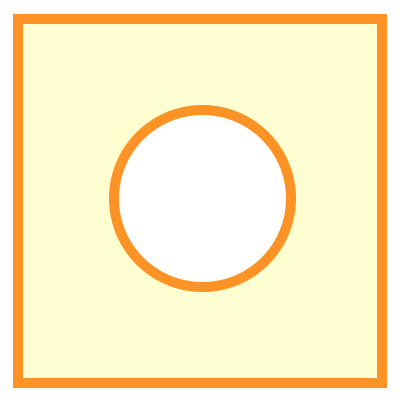
\includegraphics[width=2in]{squareminuscircle.png}
\end{figure}

}


\frame{ \frametitle{Neighborhoods in Higher Dimensions: Square}

A \textbf{square neighborhood} around $x \in \R^n$ is, for any $\delta > 0$, 
\[ (x_1 - \delta, x_1 + \delta) \times (x_2 - \delta, x_2 + \delta) \times \cdots \times (x_n - \delta, x_n + \delta). \]

Either definition of neighborhood works to describe interior points, and therefore for describing open sets: 
\begin{align*}
S \subseteq \R^n & \text{ is open } \\
 & \iff \forall x \in S, \, \exists \text{ a circular neighborhood of } x \text{ contained in } S \\
 & \iff \forall x \in S, \, \exists \text{ a square neighborhood of } x \text{ contained in } S.
\end{align*}

}


\frame{ \frametitle{Boxes in Several Dimensions}

In general, an \textbf{open rectangular region (box)} in $\R^n$ is an open set 
\[ (a_1, b_1) \times (a_2, b_2) \times \cdots \times (a_n, b_n). \]

\vspace{5mm}

Likewise, a \textbf{closed rectangular region (box)} in $\R^n$ is a closed set 
\[ [a_1, b_1] \times [a_2, b_2] \times \cdots \times [a_n, b_n]. \]

}


\frame{ \frametitle{Volume in Several Dimensions}

For a rectangular region (box) 
\[ R = [a_1, b_1] \times [a_2, b_2] \times \cdots \times [a_n, b_n], \]
define the \textbf{volume} of $R$ as 
\[ vol(R) = \prod_{i=1}^n (b_i - a_i). \]

\vspace{3mm}

\begin{itemize}
\item In $\R$, this is interval length. 

\vspace{3mm}

\item In $\R^2$ this is rectangular area.

\vspace{3mm}

\item In $\R^3$ this is usual volume.

\vspace{3mm}

\item In $\R^n$ for any $n \in \N$, this is known as \textbf{Lebesgue measure}.
\end{itemize}

}


\frame{ \frametitle{Accumulation Points, Theorems in Higher Dimensions}

$x \in \R^n$ is called an \textbf{accumulation point} of $S \subseteq \R^n$ if any neighborhood around $x$ contains a point $s \in S$ where $s \neq x$. 

\vspace{5mm}

This is the same definition as for $\R$. 

}


\frame{ \frametitle{Accumulation Points, Theorems in Higher Dimensions}

In $\R^n$, we can talk about accumulation points using circular or square neighborhoods,  and many of the results are similar.

\vspace{5mm}

\begin{itemize}
\item $S \subseteq \R^n$ is closed $\iff$ $S$ contains its accumulation points.

\vspace{3mm}

\item If $R_1$, $R_2$, ... is a sequence of closed rectangular regions such that  the sequence $(R_n)$ is a \textbf{nest}, i.e. 
\[ \lim_{n \to \infty} vol(R_n) = 0, \]
then 
\[ \bigcap_{n=1}^{\infty} R_n \] 
is a singleton set.

\vspace{3mm}

\item \textbf{Bolzano-Weierstrass Theorem}: A bounded, infinite set $S \subseteq \R^n$ contains at least one of its accumulation points.
\end{itemize}

}


\frame{ \frametitle{Neighborhoods in Higher Dimensions: Norm}

\begin{defn}
A \textbf{norm} on a vector space\footnote{leaving out some technical details; see linear algebra notes} $A$ is a function 
\[ || \cdot ||: A \to \R, \] 
generalizing the notion of ``length'', that satisfies the following properties: for any $x, y \in A$, and $c \in \R$, 

\vspace{3mm}

\begin{itemize}
\item $||0|| = 0$ (a point with length 0 is the zero vector)

\vspace{3mm}

\item $||x|| \geq 0$ (lengths are positive) 

\vspace{3mm}

\item $||cx|| = |c| \cdot ||x||$ (scaling a vector is linear)

\vspace{3mm}

\item $||x+y|| \leq ||x|| + ||y||$ (Triangle Inequality) 
\end{itemize}
\end{defn}

}


\frame{ \frametitle{Neighborhoods in Higher Dimensions: Metric}

\begin{defn}
A \textbf{metric} on a vector space $A$ is a function $d: A \times A \to \R$ (generalizing ``distance'') that satisfies, for any $x, y, z \in A$, 

\vspace{3mm}

\begin{itemize}
\item $d(x,x) = 0$ (a point is distance 0 from itself)

\vspace{3mm}

\item $d(x,y) \geq 0$ (distances are positive) 

\vspace{3mm}

\item $d(x,y) = d(y,x)$ (symmetry)

\vspace{3mm}

\item $d(x, z) \leq d(x,y) + d(y,z)$ (Triangle Inequality) 
\end{itemize}
\end{defn}

}


\frame{ \frametitle{Metric from Norm}

A norm $||\cdot||$ induces a metric by 
\[ d(x,y) = ||x - y||. \]

Neighborhoods are defined by a distance called a \textbf{radius} and a point called the \textbf{center}.

\vspace{5mm}

The most common norm used, the $L^2$ (``Euclidean'') norm, \\
induces the Euclidean metric\footnote{and the Pythagorean Theorem}
\[ d(x, y) = ||x-y||_2 = \left( \sum_{i=1}^n |x_i - y_i|^2 \right)^{1/2} \]
and generates circular neighborhoods.


}


\frame{ \frametitle{Different Metrics from Different Norms}

\begin{itemize}
\item The $L^{\infty}$ (``supremum'') norm induces the metric 
\[ d(x, y) = ||x-y||_{\infty} = \sup_{i=1,...,n}\{ |x_i - y_i| \} \]
and generates square neighborhoods.

\vspace{5mm}

\item The $L^1$ (``taxicab'', ``Manhattan'') norm induces the metric 
\[ d(x, y) = ||x-y||_1 = \left( \sum_{i=1}^n |x_i - y_i| \right) \]
and generates a different kind of square neighborhood.
\end{itemize}

}


\frame{ \frametitle{Neighborhoods in Higher Dimensions: Different Metrics}

A metric is induced by a norm is \textbf{shift-invariant}: 
\[ \forall x, y, z \in A, \,\, d(x,y) = d(x-z, y-z). \]

\vspace{3mm}

In general, for $p > 0$, the $L^p$ metric is defined by 
\[ d(x, y) = ||x-y||_p = \left( \sum_{i=1}^n |x_i - y_i|^p \right)^{1/p}. \]

\vspace{3mm}

The space denoted $L^p(\R^n)$ is generated by open ``balls'' of the form 
\[ B_{\varepsilon}(x) = \left\{ y \in \R^n: \,\, d(x,y) < \varepsilon \right\} = \left\{ y \in \R^n: \,\, ||x-y||_p^p < \varepsilon^p \right\}. \]

}


\frame{ \frametitle{Topology}

We can generalize the concept of ``open set'' away from distance.

\vspace{3mm}

\begin{defn}
A \textbf{topology} on a set $A$ is a set $\mc{T}$ of subsets of $A$ satisfying: 

\begin{itemize}
\item $\emptyset, A \in \mc{T}$, 

\item any union of elements of $\mc{T}$ is in $\mc{T}$: for any\footnote{finite, countable, or uncountable} index set $I$,
\[ \{B_i\}_{i \in I} \subseteq \mc{T} \implies \bigcup_{i \in I}B_i \in \mc{T}. \] 

\item finite intersections of elements of $\mc{T}$ are in $\mc{T}$: 
\[ B_1, B_2, ..., B_n \in \mc{T} \implies \bigcap_{i=1}^n B_i \in \mc{T}. \] 
\end{itemize}
\end{defn}

}


\frame{ \frametitle{Topology}

If $\mc{T}$ is a topology on $A$, we call the elements of $\mc{T}$ \textbf{open sets}. 

\vspace{5mm}

\begin{ex}
The \textbf{standard topology}\footnote{due to Felix Hausdorff (1868-1942)} on $\R^n$ is the one generated by any of the sets of neighborhoods discussed earlier.
\end{ex}

}



\end{document}
